% !TEX root = ../main.tex

\section{Gaussian Processes}
\label{sec:opt:GPs}

Before introducing BO directly, we first digress to introduce Gaussian
processes (GPs) as they are an essential precursor to much of the BO literature.  
As we will show in the next section, BO relies on modeling the target with a surrogate,
which can the be used to estimate the expected value and uncertainty estimates for 
the value of a function away from points that have been evaluated.  The most common
surrogate taken in the BO literature is a GP and the one we will use later in Chapter~\ref{chp:bopp}, 
hence their central importance to the BO method.

Informally one can think of a GP \citep{rasmussen2006gaussian} as being a nonparametric 
distribution\footnote{Technically speaking they are stochastic processes not a distributions.} over functions.
Equivalently, one can think of it as a generalization of a Gaussian distribution
to (uncountably) infinite dimensions.  Practically, they are powerful tool for regression, classification,
and feature extraction~\citep{kuss2005assessing,lawrence2004gaussian}.  We focus here on regression as it is generally
the simplest usage and the most relevant to our needs.

\subsection{Function-Space View}
\label{sec:opt:GPs:function}

A GP is fully specified by a mean function $\mu \colon \vartheta \rightarrow \real$ and covariance function 
$k \colon \vartheta \times \vartheta \rightarrow \real$, the latter of which must be a bounded 
$\left(\text{i.e. }k\left(\theta,\theta'\right)<\infty, \; \forall \theta,\theta' \in \vartheta\right)$ 
and reproducing kernel (we will return to this in depth later in Section~\ref{sec:opt:gps:weight}).  
We can informally describe a function $f$ as being distributed 
according to a GP:
\begin{align}
\label{eq:GP}
f \left(\theta\right) \sim GP \left(\mu\left(\theta\right), k\left(\theta,\theta'\right)\right)
\end{align}
which by definition means that the functional evaluations realized at any finite number of sample points is distributed according to a multivariate Gaussian. Note that the inputs to $\mu$ and $k$ need not be numeric and as such a GP can be defined over anything for which kernel can be defined.

\begin{figure}[t]
	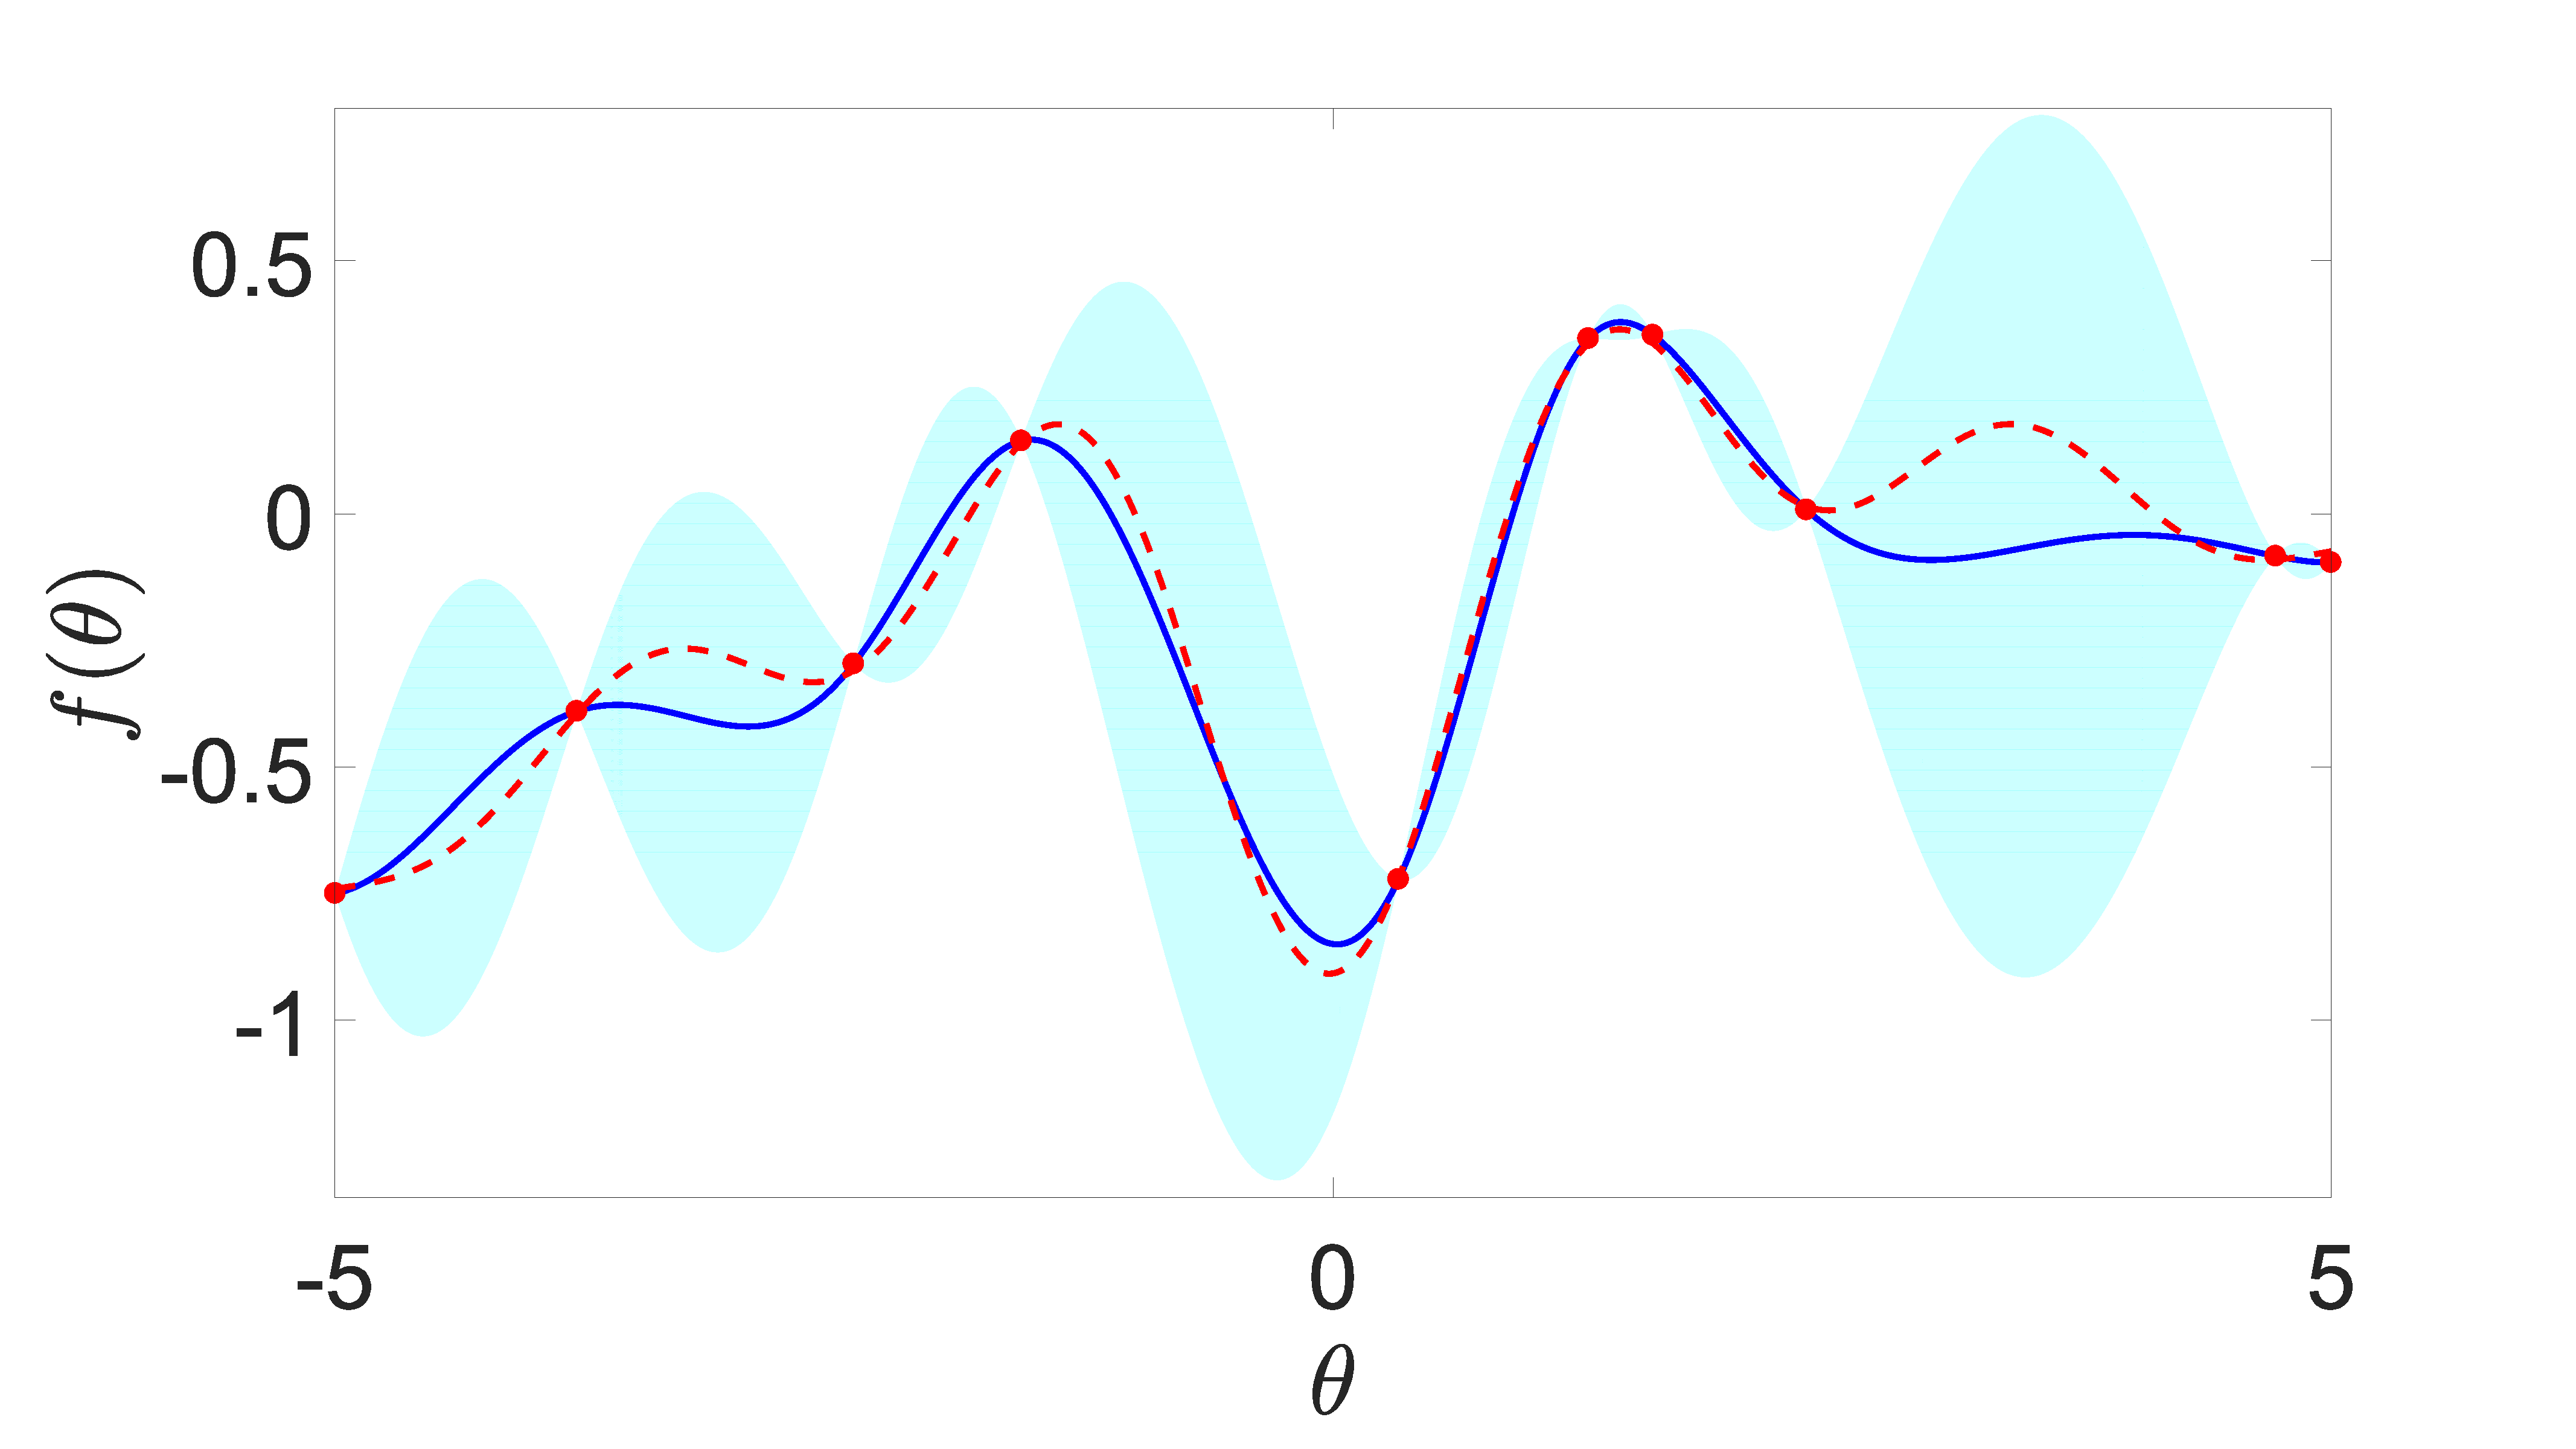
\includegraphics[width=0.48\textwidth,trim={0 0 5cm 1cm},clip]{example_gp}
		~
	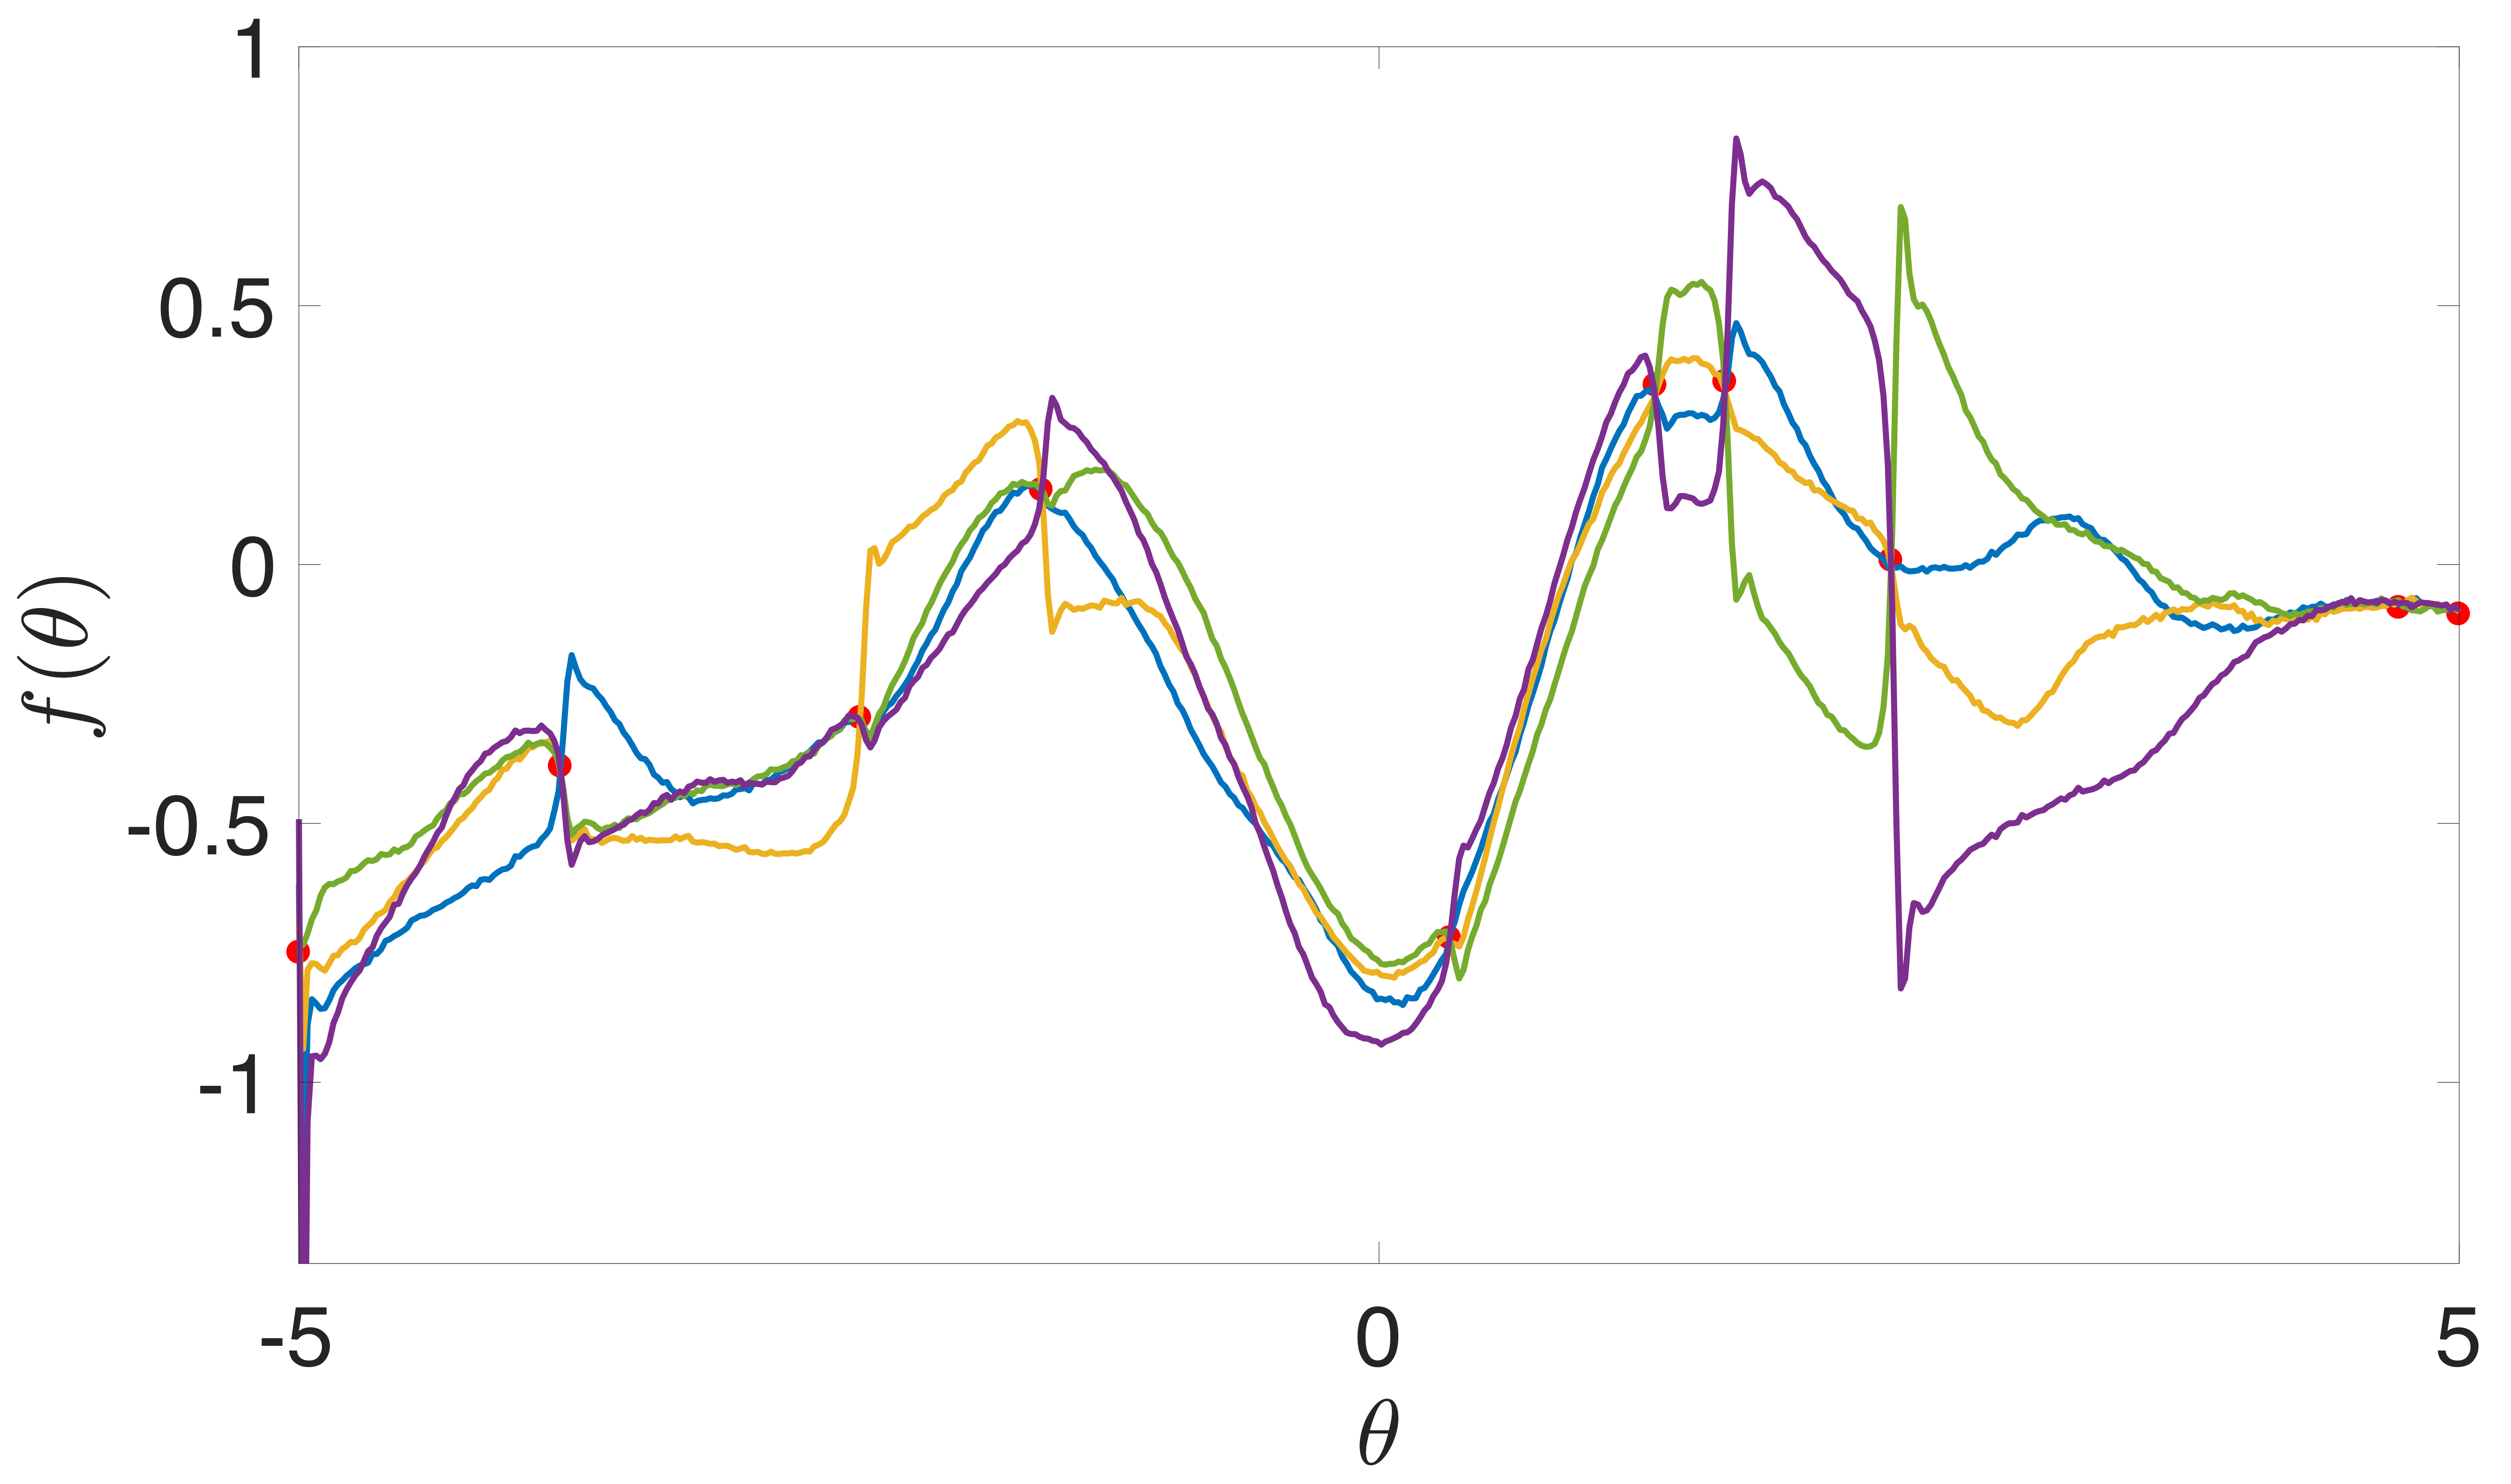
\includegraphics[width=0.50\textwidth,trim={0 0 5cm 1cm},clip]{example_functions}
	\caption{Example GP regression for points shown in left dots.  Shown left is GP where
		the solid dark blue line is the mean of the GP and the light blue shading is the
		mean $\pm2$ standard deviations.  Shown right is 4 example functions drawn
		from the GP with covariance function as per~\eqref{eq:opt:kprior}.\label{fig:opt:example_gp}}
\end{figure}

Figure~\ref{fig:opt:example_gp} shown an example GP regression with a small
number of data points $\{\theta_j,{v}_j\}_{j=1:m}$.  Here we wish to regress a function $f$ 
from $\theta$ to $y$.  To do this, we place a GP prior on $f$
\[
f_{\text{prior}} (\theta) \sim \text{GP}\left(\mu_{\text{prior}} (\theta),k_{\text{prior}}(\theta,\theta')\right),
\]
and take $\mu_{\text{prior}} (\theta) = 0 \; \forall \theta$, noting the
generality of this choice as one can simply regress $y-\mu_{\text{prior}}(\theta)$ if
a different $\mu_{\text{prior}}$ is desired.  We further take for the covariance function
\begin{align}
\label{eq:opt:kprior}
\begin{split}
k_{\text{prior}}\left(\theta,\theta'\right) = & \sigma_{3/2}^2 \left(1+\sqrt{3} \; \frac{\theta-\theta'}{\rho_{3/2}}\right)\exp\left(-\sqrt{3} \;\frac{\theta-\theta'}{\rho_{3/2}}\right) +\\&\sigma_{5/2}^2 \left(1+\sqrt{5}\;\frac{\theta-\theta'}{\rho_{5/2}}+\frac{5}{3}\left(\frac{\theta-\theta'}{\rho_{5/2}}\right)^2\right)\exp\left(-\sqrt{5}\;\frac{\theta-\theta'}{\rho_{5/2}}\right)
\end{split}
\end{align}
which corresponds to a combination of a Mat\'{e}rn-3/2 and Mat\'{e}rn-5/2
kernel with hyperparameters $\sigma_{3/2}, \sigma_{5/2}, \rho_{3/2},$ and
$\rho_{5/2}$.  We will return to how to choose the kernel function and
these parameters later, the latter of which are set to
$\sigma_{3/2}=0.04, \sigma_{5/2}=0.47, \rho_{3/2}=1.89,$ and
$\rho_{5/2}=0.98$ in Figure~\ref{fig:opt:example_gp}.  For now, we simply note
that the choice of covariance function and its parameters will heavily influence 
the nature of functions generated by the GP, dictating things such as smoothness 
and characteristic lengths scales of variation.

An important property of a GP that we now exploit is that it is conjugate with a 
Gaussian likelihood.
Let ${\Theta} = \{\theta_j\}_{j=1:m}$ and ${V} = \{{v}_j\}_{j=1:m}$ 
be the set of observed inputs and outputs respectively.
We use a separable Gaussian likelihood function
\begin{align}
\label{eq:opt:GP-lik}
p({V}| {\Theta}, f) = \prod_{j=1}^{m}p({v}_j | f(\theta_j)) = \prod_{j=1}^{m}\frac{1}{\sigma_{n}\sqrt{2\pi}} \exp \left(-\frac{\left({v}_j-f(\theta_j)\right)^2}{2\sigma_n^2}\right)
\end{align}
where $\sigma_n$ is an observation noise, set to $0.001$ in our example.  Combining this with the GP prior
we previously defined leads to GP process posterior and predictive distribution.
To see this we can consider the joint distribution between the points we have
considered so far, and a new set of points $\{{\Theta}^*,{V}^*\}$.
Introducing the shorthand $k_{\text{prior}}({\Theta},{\Theta}^*) = \left[\begin{smallmatrix} k_{\text{prior}}(\theta_1,\theta_1^*) & k_{\text{prior}}(\theta_1,\theta_2^*) & \dots\\ k_{\text{prior}}(\theta_2,\theta_1^*) & k_{\text{prior}}(\theta_2,\theta_2^*) & \dots \\ \dots & \dots & \dots\end{smallmatrix}\right]$ then we have by the fact that
any finite realisations of points is Gaussian
\begin{align}
\label{eq:opt:GP-joint}
\left[\begin{matrix} 
V \\ f^*
\end{matrix}\right] \sim \mathcal{N} \left(\mathbf{0}, \left[
\begin{matrix}
k_{\text{prior}}({\Theta},{\Theta})+\sigma_n^2 I & k_{\text{prior}}({\Theta},{\Theta}^*) \\
k_{\text{prior}}({\Theta}^*,{\Theta}) & k_{\text{prior}}({\Theta}^*,{\Theta}^*)
\end{matrix}
\right]\right)
\end{align}
where $I$ is the identity matrix, $\mathbf{0}$ is a vector of zeros, and $f^*$ is the true
function values at ${\Theta}^*$ (such that $V^*-f^*\sim\mathcal{N}(0,\sigma_n^2 I)$).
We can now use standard results for Gaussians (see e.g.~\cite{petersen2008matrix}) to get
the conditional distribution for $f^*$ given all the other variables
\begin{align}
\label{eq:opt:GP-posterior}
\begin{split}
f^* | \Theta, V, \Theta^* &\sim \mathcal{N}\left(\mu_{\text{post}} \left(\Theta^*\right), 
k_{\text{post}} \left(\Theta^*,\Theta^*\right) \right) \quad \text{where} \\
\mu_{\text{post}}  \left(\Theta^*\right) & = k_{\text{prior}}\left(\Theta^*,{\Theta} \right) \left[k_{\text{prior}}\left({\Theta} ,{\Theta}  \right) + \sigma_n^2 I\right]^{-1} V\\
k_{\text{post}} \left(\Theta^*,\Theta^*\right) & = k_{\text{prior}} \left(\Theta^*,\Theta^*\right) - k_{\text{prior}}\left(\Theta^*,{\Theta} \right) \left[k_{\text{prior}}\left({\Theta},{\Theta} \right) + \sigma_n^2 I\right]^{-1} k_{\text{prior}}\left({\Theta} ,\Theta^*\right).
\end{split}
\end{align}
Now as $\Theta^*$ are arbitrary points, this corresponds to our predictive distribution.
Further, as the predictive distribution is still a GP, we can refer to our
model as having a GP posterior
\[
f_{\text{post}} (\theta) | \Theta, V \sim \text{GP}\left(\mu_{\text{post}} (\theta),k_{\text{post}}(\theta,\theta')\right).
\]
Going back to Figure~\ref{fig:opt:example_gp}, we see the result of this process.
Our GP regression gives us a posterior mean function that represents the expected value
at every possible input points, along with a variance that represents our subjective
uncertainty in the value of the function at that point.  It is important to note that, as is
always the case in Bayesian modeling, these uncertainty estimates are generally  an underestimate,
as they do not account for the ``unknown unknowns''.  Figure~\ref{fig:opt:example_gp} also
shows that we can draw from the GP by choosing some set of evaluation points $\Theta^*$ and
then drawing from~\eqref{eq:opt:GP-posterior}.  We see that there is larger variation in the
function values away from the points that have been evaluated, as would be expected.

An important point of note is that the marginal likelihood for our model is also analytic, namely
\begin{align}
\label{eq:opt:GP-ML}
\begin{split}
\log p(V | \Theta) = &-\frac{1}{2} V^T \left[k_{\text{prior}}\left({\Theta} ,{\Theta}  \right) + \sigma_n^2 I\right]^{-1} V
-\frac{1}{2} \log \left|k_{\text{prior}}\left({\Theta} ,{\Theta}  \right) + \sigma_n^2 I\right|-\frac{m}{2} \log 2\pi
\end{split}
\end{align}
where $m$ is the number of points in $\Theta$.  This is important as it means it will be tractable to
optimize or do inference over the GP hyperparameters.

\subsection{Kernels and Hyperparameters}
\label{sec:opt:gps:kernels}

As we showed in the last section, GPs form powerful and expressive priors over functions.
In this section we show that their practical behavior varies substantially depending on the
choice of the covariance function, aka kernel, and the hyperparameters.   Informally, we can think
of the kernel as expressing the similarity between the evaluation of the function at two different input
points $\theta$ and $\theta'$.  When $k(\theta,\theta')$ is large, these evaluations are strongly
correlated such that the evaluations will have similar values.  When it is small, there is little
correlation between the points and so their evaluations will be roughly independent.  Note that
it is possible for $k(\theta,\theta')<0$ provided $\theta\neq\theta'$, but as kernels must
be positive definition functions as explained in the next section, $k\left(\Theta,\Theta\right)$ is
always a positive definite matrix.  Though it is not necessary for the kernel to be stationary (i.e.
that it only depends on $\theta-\theta'$ rather than the absolute values), we will not
consider non-stationary cases further here (see \cite{rasmussen2006gaussian} for further
information).
%
%\begin{figure}[t]
%	\centering
%	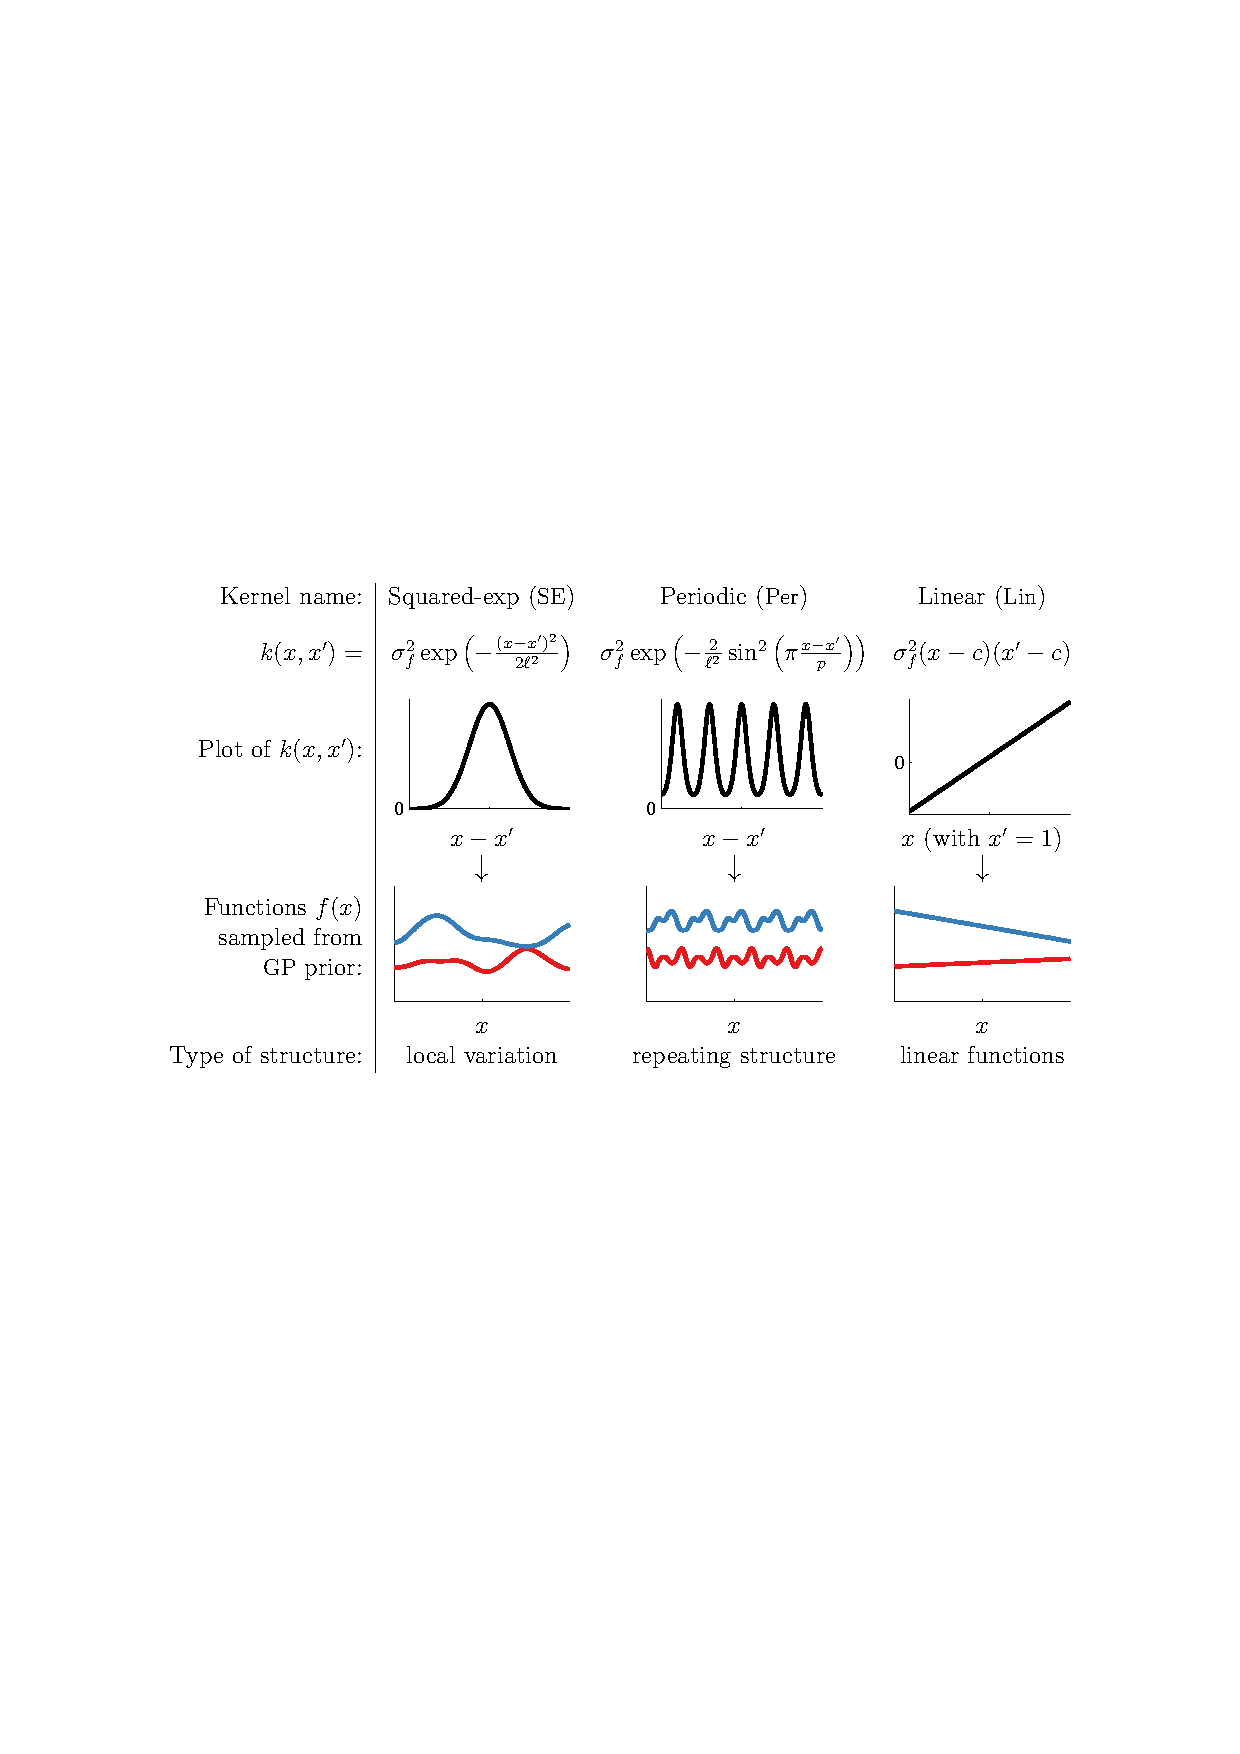
\includegraphics[width=0.95\textwidth]{example_kernels}
%	\caption{Example basic kernels.  Figure taken from David Duvenaud's PhD
%		Thesis. \label{fig:opt:example_kernels_duv}}
%\end{figure}

\cite[Figure 2.1]{duvenaud2014automatic} shows
some simple example kernels.  Note $x$ here is equivalent to $\theta$ in our
notation.  The figure shows that the qualitative behavior of the GP changes
substantially with changes to the kernel.  All of these kernels also behave
substantially differently to the compound Mat\'{e}rn kernel we considered in the last section.
The choice of kernel is therefore
critical to the performance of GPs.  Though there is work, including some of
our own~\citep{janz2016probstruct}, that examines methods 
for learning the kernel directly
\citep{duvenaud2013structure,lloyd2014automatic,wilson2014fast}, 
this is typically too computationally intensive
to carry out in practice.  One must therefore either use prior knowledge about the
problem, or use an relatively general purpose kernel to ensure that the nuances of the
data are not overwhelmed.

A particularly common problem in the choice of kernel is in the desired level
of smoothness.  At the one extreme, one can use the squared exponential kernel
\begin{align}
\label{eq:opt:se-kernel}
k_{\text{se}} \left(\theta,\theta'\right) = \sigma_f^2 \exp \left(-\frac{\left\lVert \theta - \theta'\right\rVert^2_2}{2 \rho^2}\right)
\end{align}
which is infinitely differentiable.   Here $\sigma_f^2$ is the ``signal 
standard deviation'' -- a hyperparameter that
affects the scaling of the output from the GP: the larger $\sigma_f$, the higher
the average standard deviation of the function.  Meanwhile, $\rho$ is a hyperparameter
that dictates the characteristic length scale of variation for the function -- the
higher $\rho$ is, the slower the correlation decreases as one moves away from the
current point, and therefore the less ``wiggly'' the function is.  Both these
hyperparameters are shared by most commonly used kernels.  Although the
presented kernel is isotropic, this is easily relaxed by having a different $\rho$
for each dimension.

\begin{figure}[t]
	\centering
	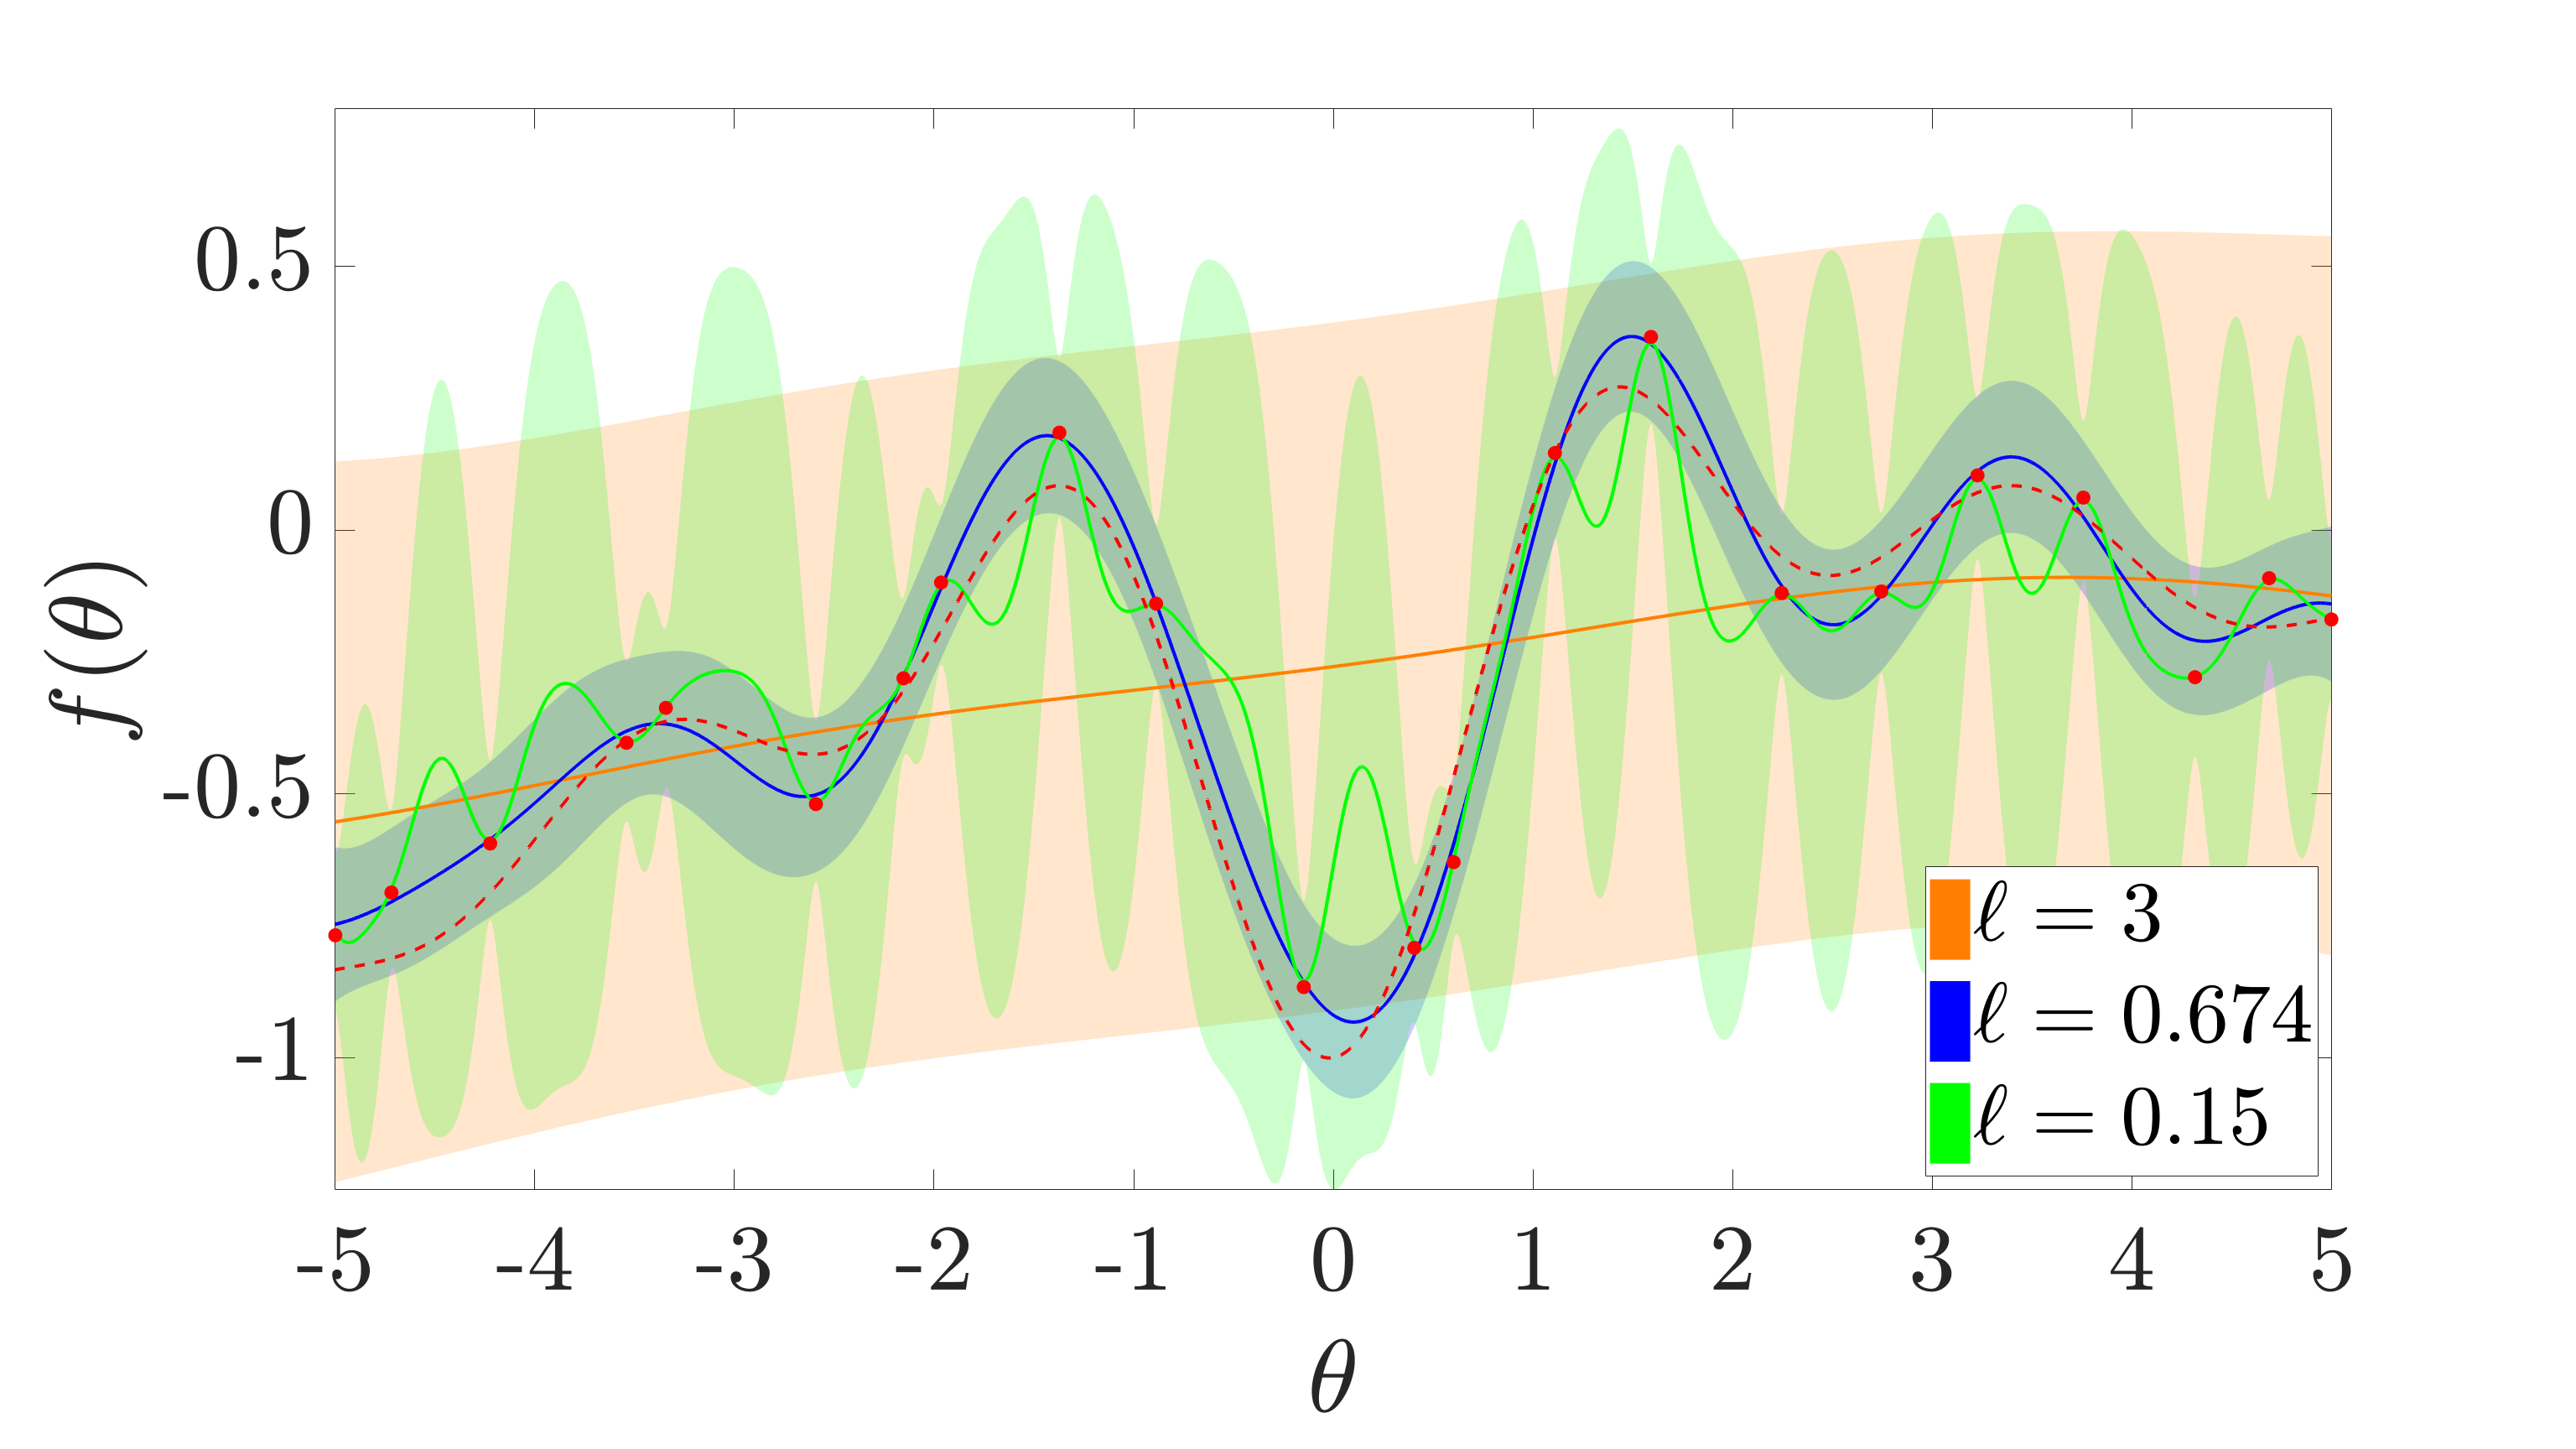
\includegraphics[width=0.6\textwidth]{hyper-changes}
	\caption{Effective of changing the length scale for Mat\'{e}rn-5/2 kernel.\label{fig:opt:hyper-changes}}
\end{figure}

In many practical problems, the squared exponential kernel is too smooth.
One possible alternative in these scenarios are the Mat\'{e}rn kernels.  The
Mat\'{e}rn-$\nu$ kernel, given by
\begin{align}
k_{\nu}\left(\theta,\theta'\right) = \sigma_f \frac{2^{1-\nu}}{\Gamma\left(\nu\right)}\left(\frac{\sqrt{2\nu}}{\rho}\left\lVert\theta-\theta'\right\rVert\right)^{\nu} K_\nu
 \left(\frac{\sqrt{2\nu}}{\rho}\left\lVert\theta-\theta'\right\rVert\right)
\end{align}
where $K_{\nu}$ is the modified Bessel function of second kind order $\nu$
and $\Gamma(\cdot)$ is the gamma function,
is $\lfloor\nu-1\rfloor$ times differentiable and
therefore different values of $\nu$ can be used to express different levels
of smoothness.  Typically $\nu$ is set to $n+1/2$ for some integer $n$, for
which is has a simple closed form~\citep{rasmussen2006gaussian}.

Though the choice of kernel function is critical for a GP, the choice of
hyperparameters such as the scaling and length scale can have equally
significant impact on the behavior.  Figure~\ref{fig:opt:hyper-changes} shows
the effect of changing the length scale of a Mat\'{e}rn-5/2 kernel.  When the length
scale is too large as shown in orange, the regressed function is overly smooth and
does not capture the data.  When the length scale is too small, as shown in green,
wild fluctuations are permitted in between the datapoints such that there is very
high uncertainty between points and also potentially overfitting as the regressor
can model all the fluctuations in the data, including those originating simply from
noisy evaluations.
As the hyperparameters are rarely known upfront, one must typically either optimize
them, or perform inference over them to produce a mixture of GPs.

\subsection{Weight-Space View and Reproducing Kernel Hilbert Space}
\label{sec:opt:gps:weight}

One of the key advantages of GPs is that they can be used effectively without needing
to know the intricacies for why they work.  The derivations we introduced in the
last section and in particular the calculations required to derive the GP posterior were
spectacularly simple, albeit computationally intensive (the need for a matrix inversion
to calculate~\eqref{eq:opt:GP-posterior} means that training is $O(m^3)$ for
$m$ training points).  However, what is going on beneath the surface is substantially
more complicated, which is perhaps not surprising when one remembers that they
are defined over uncountably infinitely many variables.  
To truly understand the underlying rational and assumptions for GPs, and to properly
appreciate the restrictions on possible kernels, it is necessary to delve into GPs more
formally, taking a so-called weight-space view.
In this section we therefore outline a more formal derivation of a GP
from the viewpoint of reproducing kernels \citep{hofmann2008kernel}
and show how they can be thought of as Bayesian linear regression
using an infinite number of features.
We start with the following definitions.

\begin{definition}{}
	An inner product $\langle\cdot,\cdot\rangle_{\mathcal{H}}$ is a function $\mathcal{H} \times \mathcal{H} \rightarrow \real$ 
	associated with a vector space $\mathcal{H}$
	that is symmetric $\langle u,v\rangle_{\mathcal{H}}=\langle v,u\rangle_{\mathcal{H}}$, linear $\langle a u_1 + b u_2,v\rangle_{\mathcal{H}} = a \langle u_1,v\rangle_{\mathcal{H}} +b\langle u_2,v\rangle_{\mathcal{H}}$, and positive definitive $\langle u,u\rangle_{\mathcal{H}} \ge 0, \; \langle u,u\rangle_{\mathcal{H}} = 0 \; \Leftrightarrow \; u=\mathbf{0}$.
	\label{opt:def:InnerProduce}
\end{definition}
\begin{definition}{}
	A Hilbert space, $\mathcal{H}$, is a, potentially uncountably infinite, vector space associated with an inner product
	$\langle\cdot,\cdot\rangle_{\mathcal{H}}$ 
	which is complete with respect to the norm $\norm{u}_{\mathcal{H}} = \sqrt{\langle u,u\rangle_{\mathcal{H}}}$.
	\label{opt:def:HilbertSpace}
\end{definition}
\noindent Less formally, we can think of Hilbert spaces as being a generalization of Euclidean space (i.e. the space vectors live in)
to include functions.  Using Hilbert spaces, we can think of a function as being an uncountably long vector defining
the value of the function at each possible input point.

Consider now the linear (in the weights $\mathbf{w}$) model
\begin{align}
\label{eq:opt:linModel}
f \left(\theta\right) = \mathbf{w}^T Z \left(\theta\right)  + \mu\left(\theta\right), \quad \mathbf{w} \sim \mathcal{N} \left(\mathbf{0}, C\right)
\end{align}
where $Z\left(\cdot\right) = \left[\zeta_1\left(\cdot\right),\dots,\zeta_m\left(\cdot\right)\right]^T, \; \zeta_a \colon \vartheta \rightarrow \real$ for $a = 1,\dots,m$ is a feature map in $m$-dimensional Hilbert space $\mathcal{H}$.  For any set of points $\theta_1,\dots,\theta_t$ then $F = \left[f\left(\theta_1\right),\dots,f\left(\theta_t\right)\right]^T$ will be distributed according to a $t-$dimensional Gaussian with mean $\left[\mu\left(\theta_1\right),\dots,\mu\left(\theta_t\right)\right]^T$ and covariance $k\left(\theta_i,\theta_j\right) = Z\left(\theta_i\right)^T C Z\left(\theta_j\right), \; \forall i,j \in \left\{1,\dots,t\right\}$.  Note that 
\begin{align}
\label{eq:opt:poskernel}
Z\left(\theta\right)^T C Z\left(\theta'\right) = \sum_{a=1}^{m} \sum_{b=1}^{m} C_{ab}\zeta_a\left(\theta\right)\zeta_b\left(\theta'\right) \ge 0, \quad \forall \theta, \theta' \in \vartheta
\end{align}
as $C$ must be positive semi-definite for the distribution on $\mathbf{w}$ to be well defined\footnote{$Z\left(\theta_i\right)^T C Z\left(\theta_j\right)=0$ is only possible if $\mathbf{w}$ lives in a lower dimensional subspace of $\real^m$}.  This also means that the Cholesky decomposition $C^{1/2}$ exists and we can define $\Psi\left(\cdot\right) = C^{1/2} Z\left(\cdot\right) = \left[\psi_1\left(\cdot\right),\dots,\psi_m\left(\cdot\right)\right]^T$ to give a covariance function $k \colon \vartheta \times \vartheta \rightarrow \real$ of the form
\begin{align}
\label{eq:opt:covFunc}
k\left(\theta,\theta'\right) = \langle\Psi\left(\theta\right), \Psi\left(\theta'\right)\rangle_{\mathcal{H}} = \sum_{a=1}^{m} \psi_a\left(\theta\right) \psi_a\left(\theta'\right) \le \sqrt{\sum_{a=1}^{m} \left(\psi_a\left(\theta\right)\right)^2} \sqrt{\sum_{a=1}^{m} \left(\psi_a\left(\theta'\right)\right)^2}
\end{align}
where the inequality trivially follows using Cauchy-Schwarz.  Now consider the case were $m$ is uncountably infinite such that $\mathcal{H}$ represents a functional space along with an inner product.  If $\Psi \left(\cdot\right)$ remains 
in $L^2$ space, i.e.
\begin{align}
\label{eq:opt:l2Space}
\sum_{a=1}^{\infty} \left(\psi_a\left(\theta\right)\right)^2 < \infty, \quad \forall \theta \in \vartheta,
\end{align}
then $k\left(\theta,\theta'\right) < \infty, \; \forall \theta, \theta' \in \vartheta$ using the inequality from equation \eqref{eq:opt:covFunc}, and our covariance will remain bounded with infinitely many basis functions.

The key realization is now that the distribution of $F$ only depends on $Z$ and $C$ through the inner product
$\langle\Psi\left(\theta\right), \Psi\left(\theta'\right)\rangle_{\mathcal{H}}$ such that we need never compute 
the (potentially infinite) mapping $\Psi\left(\theta\right)$ if we can find a way to implicitly compute the inner product, 
for example if $k$ has the \emph{reproducing property}
\begin{align}
\label{eq:opt:repKernel}
\langle u \bc, k\left(\cdot,\theta\right)\rangle_{\mathcal{H}} = u\left(\theta\right), \quad \forall \theta \in \vartheta, \; \forall u\bc \in \mathcal{H}.
\end{align}
This is called the kernel trick, where we have used the representation $\Psi\left(\theta\right) = k\left(\cdot,\theta\right)$ noting that any feature map can be thought of as parameterizing a mapping $\mathcal{H} \rightarrow \real$ through the inner product.
We can now introduce the notion of \emph{reproducing kernel Hilbert space} (RKHS) \citep{aronszajn1950theory}.
\begin{definition}{}
	\label{def:opt:RKHS}
	Given a Hilbert space $\mathcal{H}$, then a function $k \colon \vartheta \times \vartheta \rightarrow \real$ is a reproducing
	kernel and  $\mathcal{H}$ is a reproducing kernel Hilbert space if
	$k\left(\cdot,\theta\right) \in \mathcal{H}, \; \forall \theta \in \vartheta$ and the reproducing property described in equation \eqref{eq:opt:repKernel} is satisfied.
\end{definition}
\noindent The significance of RKHSs for GPs is that their covariance functions correspond to reproducing kernels and
so a GP is defined over a RKHS.  Most RKHSs do not contain all possible functions -- e.g. the RKHS associated
with the squared exponential kernel contains only infinitely differentiable functions -- and so the choice
of GP kernel will dictate the range functions it is capable of encapsulating.
Note that as $k\left(\theta,\theta'\right) = \left\langle k\left(\cdot,\theta\right), k\left(\cdot,\theta'\right)\right\rangle = k\left(\theta',\theta\right)$, all reproducing kernels are symmetric.

Going back to our GP derivation, then for the realization of $k\left(\theta,\theta'\right)$ at a finite number of points to be a valid covariance matrix we further require it to be positive definite, i.e:
\begin{align}
\label{eq:opt:posDef}
\sum_{i=1}^{n} \sum_{j=1}^{n} \beta_i \beta_j k\left(\theta_i,\theta_j\right) \ge 0, \quad \forall n \ge 1, \; \forall \left\{\beta_1, \dots, \beta_n \right\}  \in \real^n, \; \forall \left\{\theta_1, \dots, \theta_n \right\} \in \vartheta^n
\end{align}
which can be proved to be the case given the restrictions we have placed on $k$ by noting
\begin{align}
\label{eq:opt:posDefProof}
\sum_{i=1}^{n} \sum_{j=1}^{n} \beta_i \beta_j k\left(\theta_i,\theta_j\right) = \sum_{i=1}^{n} \beta_i {\Psi\left(\theta_i\right)}^T \sum_{j=1}^{n} \beta_j \Psi\left(\theta_j\right) = \left\lVert \sum_{i=1}^{n} \beta_i \Psi\left(\theta_i\right) \right\rVert^2_\mathcal{H} \ge 0.
\end{align}
Consequently, \eqref{eq:opt:l2Space} is a sufficient condition for the distribution of $F$ to be a multivariate $t-$dimensional Gaussian with a valid and finite covariance matrix when we consider an uncountable infinite number of basis functions.  Furthermore, we note that many choices for $\Psi$ will lead to closed form analytic expressions of $\langle\Psi\left(\theta\right), \Psi\left(\theta'\right)\rangle_{\mathcal{H}}$ without the need to ever calculate $\Psi\left(\theta\right)$ explicitly.  

To show a simple example of this consider the one-dimensional case were $\theta \in \real$ and basis functions of the form  $\psi_a = \sigma_w\exp \left(-\frac{\left( \theta-c_a\right)^2}{2 \rho^2}\right)$ where $c_a \in \left[c_{\min},c_{\max}\right]$ represents the center of the basis function and $\rho$ is a common length scale.  Further specify that $\sigma_w^2 = \frac{\beta \left(c_{\max}-c_{\min}\right)}{m}$, i.e. that $\sigma_w^2$ is proportional to the number of functions per unit length, then we have
\begin{align}
\label{eq:opt:kSeqExpFinite}
k\left(\theta,\theta'\right) = \sum_{a=1}^{m} \frac{\beta \left(c_{\max}-c_{\min}\right)}{m} \exp \left(-\frac{\left( \theta-c_a\right)^2}{2 \rho^2}\right) \exp \left(-\frac{\left(\theta'-c_a\right)^2}{2 \rho^2}\right).
\end{align}
If we assume that the basis functions are evenly space in $\left[c_{\min},c_{\max}\right]$, then in the limit $m \rightarrow \infty$
we recover the integral
\begin{align}
\label{eq:opt:kSeqExpIntegral}
k\left(\theta,\theta'\right) = \beta \int_{c_{\min}}^{c_{\max}}  \exp \left(-\frac{\left( \theta-c\right)^2}{2 \rho^2}\right) \exp \left(-\frac{\left(\theta'-c\right)^2}{2 \rho^2}\right) dc.
\end{align}
Now if we further take $c_{\min} \rightarrow -\infty$ and $c_{\max} \rightarrow \infty$ then we have the analytic solution
\begin{align}
\label{eq:opt:seqExpProof}
k\left(\theta,\theta'\right) = \sqrt{\pi} \rho \beta \exp \left(-\frac{\left(\theta-\theta'\right)^2}{4 \rho^2}\right).
\end{align}
which is the common squared exponential kernel in one dimension.  Thus we have managed to analytically marginalize over all basis functions and are left with a simple expression that can be used to evaluate the covariance between any two given points that implicitly uses an uncountably infinite number of basis functions.

More generally, the Moore-Aronszajin theorem \citep{aronszajn1950theory} states that
\begin{theorem}
	\label{the:opt:Moore-Aronszajin}
	Any symmetric, positive definite kernel $k \colon \vartheta \times \vartheta \rightarrow \real$ has a unique RKHS for which $k$ is a reproducing kernel.
\end{theorem}
\noindent In other words, if we define a kernel function that is symmetric $k\left(\theta,\theta'\right) = k\left(\theta',\theta\right)$ and positive definite as per \eqref{eq:opt:posDef}, then at least one corresponding feature map $\Psi \colon \vartheta \rightarrow \mathcal{H}$ must exist.  Therefore a corresponding $Z \colon \vartheta \rightarrow \mathcal{H}$ and $C$ must also exist (for example we can trivially take $C$ as the identity matrix and $Z = \Psi$), and if we further ensure that $k$ is bounded $k\left(\theta,\theta'\right) < \infty, \; \forall \theta, \theta' \in \vartheta$, then finite realizations  $\left[f\left(\theta_1\right),\dots,f\left(\theta_t\right)\right]^T$ of equation \eqref{eq:opt:linModel} must be distributed to a finite multivariate Gaussian distribution with mean  $\left[\mu\left(\theta_1\right),\dots,\mu\left(\theta_t\right)\right]^T$ and covariance $k\left(\theta_i,\theta_j\right) \; \forall i,j \in {1,\dots,t}$.  
%
%We have therefore arrived at the following formal definition of a GP.
%
%\begin{definition}{}
%	\label{def:opt:GP}
%	A Gaussian process describes the probability distribution for the functional realisations $f \colon \vartheta \rightarrow \real$ of \eqref{eq:opt:linModel} in the limit of uncountably many basis functions, noting that this distribution is fully defined by a mean function $\mu \colon \vartheta \rightarrow \real$ and a covariance function $k\colon \vartheta \times \vartheta \rightarrow \real$, the latter of which must be a positive definite (or equivalently reproducing), bounded kernel.  
%\end{definition}{}

We can therefore think of GP regression as Bayesian linear regression using
a feature mapping to a RKHS.  This shows the power of a GP -- for appropriate
choices of kernel it uses an uncountable number of features -- but also highlights
their assumptions: the co-Gaussianity of the weights and reliance of the target
function to fall in RKHS represented by the covariance function.